 % \documentclass[11pt]{beamer}
 \documentclass[11pt,handout]{beamer}
%%%%%%%%%%%%%%%%%%%%%%%%%%%%%%%%%%%%%%%%%%%%%%%%%%%%%%%%%%%%%%%%%%%%%%%%%%%%%%%%%%%%%%%%%%%%%%%%%%%%%%%%%%%%%%%%%%%%%%%%%%%%%
% color schemes, etc
% load packages;
\usetheme{Boadilla}
% https://tex.stackexchange.com/questions/66252/placing-the-figure-exactly-at-the-top-of-the-page-in-latex
%
\makeatletter
\setlength{\@fptop}{0pt}
\makeatother
%
%%%%%%%%%%%%%%%%%%%%%%%%%%%%%%%%%%%%%%%%%%%%%%%%%%%%%%%%%%%%%%%%%%%%%%%%%%%%%%%%%%%%%%%%%%%%%%%%%%%%%%%%%%%%%%%%%%%%%%%%%%%%%
\usepackage{mathptmx}
\usepackage{amsmath}
\usepackage{amssymb}
\usepackage{graphicx}
\usepackage[export]{adjustbox}
\usepackage{subcaption}
\begin{document}
%%%%%%%%%%%%%%%%%%%%%%%%%%%%%%%%%%%%%%%%%%%%%%%%%%%%%%%%%%%%%%%%%%%%%%%%%%%%%%%%%%%%%%%%%%%%%%%%%%%%%%%%%%%%%%%%%%%%%%%%%%%%%
% define title, etc
%%%%%%%%%%%%%%%%%%%%%%%%%%%%%%%%%%%%%%%%%%%%%%%%%%%%%%%%%%%%%%%%%%%%%%%%%%%%%%%%%%%%%%%%%%%%%%%%%%%%%%%%%%%%%%%%%%%%%%%%%%%%%

\title[Volcanic Snowball Earth]{Volcanic Snowballs}
\author{Eugene Tan}
\date{\today}

% Outline 10 slides
% 1 Motivation - Pierrehumbert et al. 
% 2 Increasing Albedo puts you into disequilibrium. Regardless of whether you increase alpha 2 
% 3 ... or alpha 1
% 4 Could volcanoes have done this? They increase stratospheric Albedo (put a nice graphic). Dissipate quickly though, so need a lot of volcanoes
% 5 Physically changes your equation to modify albedo, what is the new planetary
% 6 Increasing tau puts you into a snowball. 
% 7 Draw a box model of ice cover. increasing ice extent decreases Air sea flux from lab 4 and decreases the carbon sink. 
% 8 When CO2 builds up, then B increases in our model. 
% 9 When B increases, we can get back to an partially covered equilibrium.  
% 10 Snowball means you can explain the hysteresis.

\begin{frame}{Could albedo changes explain Neoproterozoic glaciations? (Pierrehumbert et al. 2011)}
    \centering
    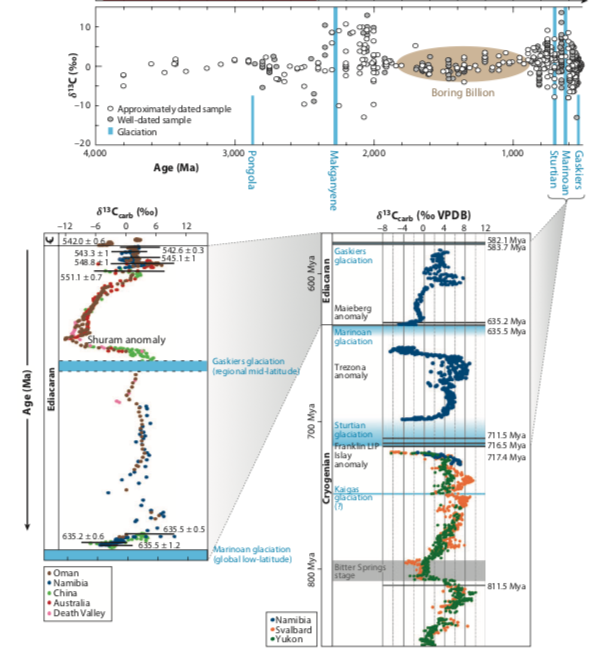
\includegraphics[width=.8\textwidth,height=.85\textheight,keepaspectratio]{img/pierrehumbert.png}
\end{frame}

\begin{frame}{Increasing land and ocean albedo can cause a snowball}
    \centering 
    \includegraphics<1 >[width=.9\textwidth,height=.9\textheight,keepaspectratio]{img/alpha1_0.png}
    \includegraphics<2 >[width=.9\textwidth,height=.9\textheight,keepaspectratio]{img/alpha1_1.png}
    \includegraphics<3 >[width=.9\textwidth,height=.9\textheight,keepaspectratio]{img/alpha1_2.png}
    \includegraphics<4 >[width=.9\textwidth,height=.9\textheight,keepaspectratio]{img/alpha1_3.png}
    \includegraphics<5 >[width=.9\textwidth,height=.9\textheight,keepaspectratio]{img/alpha1_4.png}
    \includegraphics<6 >[width=.9\textwidth,height=.9\textheight,keepaspectratio]{img/alpha1_5.png}
    \includegraphics<7 >[width=.9\textwidth,height=.9\textheight,keepaspectratio]{img/alpha1_6.png}
    % \includegraphics<8 >[width=.9\textwidth,height=.9\textheight,keepaspectratio]{img/alpha1_7.png}
    % \includegraphics<9 >[width=.9\textwidth,height=.9\textheight,keepaspectratio]{img/alpha1_8.png}
    % \includegraphics<10>[width=.9\textwidth,height=.9\textheight,keepaspectratio]{img/alpha1_9.png}
    % \includegraphics<11>[width=.9\textwidth,height=.9\textheight,keepaspectratio]{img/alpha1_10.png}
\end{frame}     
\begin{frame}{So can increasing ice albedo.}
    \centering
    \includegraphics<1 >[width=.9\textwidth,height=.9\textheight,keepaspectratio]{img/alpha2_0.png}
    \includegraphics<2 >[width=.9\textwidth,height=.9\textheight,keepaspectratio]{img/alpha2_1.png}
    \includegraphics<3 >[width=.9\textwidth,height=.9\textheight,keepaspectratio]{img/alpha2_2.png}
    \includegraphics<4 >[width=.9\textwidth,height=.9\textheight,keepaspectratio]{img/alpha2_3.png}
    \includegraphics<5 >[width=.9\textwidth,height=.9\textheight,keepaspectratio]{img/alpha2_4.png}
    \includegraphics<6 >[width=.9\textwidth,height=.9\textheight,keepaspectratio]{img/alpha2_5.png}
    \includegraphics<7 >[width=.9\textwidth,height=.9\textheight,keepaspectratio]{img/alpha2_6.png}
    \includegraphics<8 >[width=.9\textwidth,height=.9\textheight,keepaspectratio]{img/alpha2_7.png}
    % \includegraphics<9 >[width=.9\textwidth,height=.9\textheight,keepaspectratio]{img/alpha2_8.png}
    % \includegraphics<10>[width=.9\textwidth,height=.9\textheight,keepaspectratio]{img/alpha2_9.png}
    % \includegraphics<11>[width=.9\textwidth,height=.9\textheight,keepaspectratio]{img/alpha2_10.png}
\end{frame}      

\begin{frame}{A volcanic mechanism to increase albedo}
    Volcanoes put particulates into \emph{stratosphere} that increase albedo
    \centering
    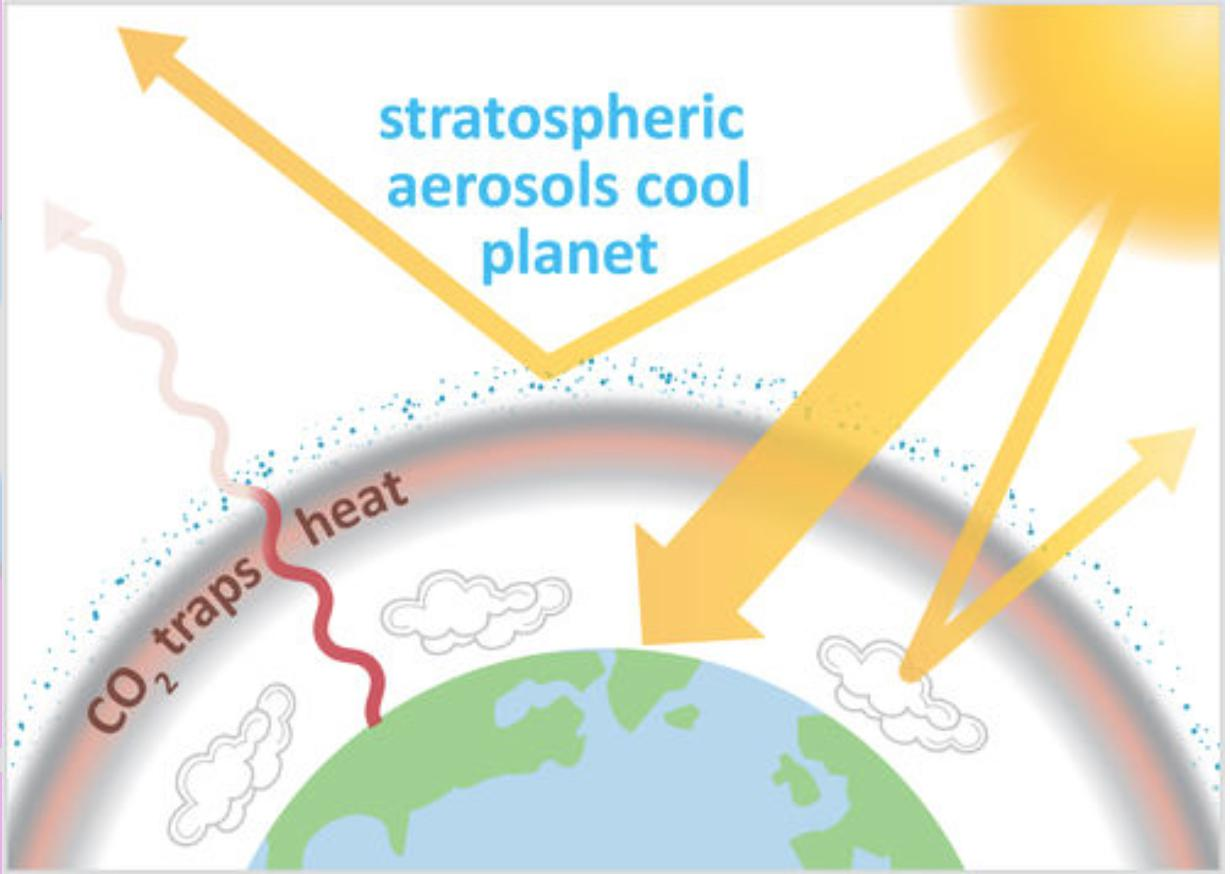
\includegraphics[width=.9\textwidth,height=.9\textheight,keepaspectratio]{img/strat_aerosol_diagram.jpg}
\end{frame}

\begin{frame}{$\tau$ is Optical Depth, $\alpha_{st}(\tau, x_s)$ is Stratospheric Albedo}
    Adapted equation from Budyko (1969)
    $$\frac{Q_0}{4} S(x_s)\textcolor{red}{(1-\alpha_{st}(x_s, \tau))}(1-\alpha_{su}(x_s)) = A + BT(x_s) + C (T(x_s)-\bar{T})$$
    \pause
    Assumption: Uniform effect over surface.
    $$1- e^{-\tau m(x)} = \alpha_{st}(x, \tau) = \alpha_{st}(\tau) = 1- e^{-\tau}$$
    \pause
    Allowing us to calculate a new planetary albedo (surface + stratosphere)
    $$ \alpha_p' = \int_0^1 S(x) [\textcolor{red}{\alpha_{st}(\tau)} + \alpha_{su}(x_s) - \textcolor{red}{\alpha_{st}(\tau)\alpha_{su}(x_s)}] dx,$$
    \pause
    Resulting in a new equation to solve (Roe and Baker 2010)
    $$\frac{Q}{4}S(x_s)(1-\alpha_{su})\textcolor{red}{(1-\alpha_{st})} + \frac{QC}{4B}(1-\textcolor{red}{\alpha_p'}) = k$$
\end{frame}

\begin{frame}{Increasing $\tau$ or $\alpha_{st}$}
    \centering
    \includegraphics<1 >[width=.9\textwidth,height=.9\textheight,keepaspectratio]{img/tau_0.png}
    \includegraphics<2 >[width=.9\textwidth,height=.9\textheight,keepaspectratio]{img/tau_1.png}
    \includegraphics<3 >[width=.9\textwidth,height=.9\textheight,keepaspectratio]{img/tau_2.png}
    \includegraphics<4 >[width=.9\textwidth,height=.9\textheight,keepaspectratio]{img/tau_3.png}
    \includegraphics<5 >[width=.9\textwidth,height=.9\textheight,keepaspectratio]{img/tau_4.png}
    \includegraphics<6 >[width=.9\textwidth,height=.9\textheight,keepaspectratio]{img/tau_5.png}
    \includegraphics<7 >[width=.9\textwidth,height=.9\textheight,keepaspectratio]{img/tau_6.png}
    % \includegraphics<8 >[width=.9\textwidth,height=.9\textheight,keepaspectratio]{img/tau_7.png}
    % \includegraphics<9 >[width=.9\textwidth,height=.9\textheight,keepaspectratio]{img/tau_8.png}
    % \includegraphics<10>[width=.9\textwidth,height=.9\textheight,keepaspectratio]{img/tau_9.png}
    % \includegraphics<11>[width=.9\textwidth,height=.9\textheight,keepaspectratio]{img/tau_10.png}
\end{frame}

\begin{frame}{Increasing  $CO_2 \approx$ increasing B}
    Ice sheets block the ocean sink for $CO_2$
    \centering
    \includegraphics<1 >[width=.9\textwidth,height=.7\textheight,keepaspectratio]{img/co2_sink/Slide1.png}
    
    \pause 
    Increasing CO2 increases $\bar{T}$, increasing OLR or B in the Budyko model.
    
    \includegraphics<2 >[width=.9\textwidth,height=.7\textheight,keepaspectratio]{img/co2_sink/Slide2.png}
    \includegraphics<3 >[width=.9\textwidth,height=.7\textheight,keepaspectratio]{img/co2_sink/Slide3.png}
    \includegraphics<4 >[width=.9\textwidth,height=.7\textheight,keepaspectratio]{img/co2_sink/Slide4.png}
     
\end{frame}

\begin{frame}{Increasing $CO_2 \rightarrow$ can get us back to a partial-ice world.}
    \centering
    \includegraphics<1 >[width=.9\textwidth,height=.9\textheight,keepaspectratio]{img/B_0.png}
    \includegraphics<2 >[width=.9\textwidth,height=.9\textheight,keepaspectratio]{img/B_1.png}
    \includegraphics<3 >[width=.9\textwidth,height=.9\textheight,keepaspectratio]{img/B_2.png}
    \includegraphics<4 >[width=.9\textwidth,height=.9\textheight,keepaspectratio]{img/B_3.png}
    \includegraphics<5 >[width=.9\textwidth,height=.9\textheight,keepaspectratio]{img/B_4.png}
    \includegraphics<6 >[width=.9\textwidth,height=.9\textheight,keepaspectratio]{img/B_5.png}
    \includegraphics<7 >[width=.9\textwidth,height=.9\textheight,keepaspectratio]{img/B_6.png}
    \includegraphics<8 >[width=.9\textwidth,height=.9\textheight,keepaspectratio]{img/B_7.png}
    \includegraphics<9 >[width=.9\textwidth,height=.9\textheight,keepaspectratio]{img/B_8.png}
    \includegraphics<10>[width=.9\textwidth,height=.9\textheight,keepaspectratio]{img/B_9.png}
    \includegraphics<11>[width=.9\textwidth,height=.9\textheight,keepaspectratio]{img/B_10.png}
\end{frame}

% 10 The partially covered equilibrium only needs to recover the carbon sink a bit in order to get back to a snowball. 
\begin{frame}{CO2 sink reactivates, causing hysteresis}
    \centering
    \includegraphics<1 >[width=.9\textwidth,height=.9\textheight,keepaspectratio]{img/Bback_0.png}
    \includegraphics<2 >[width=.9\textwidth,height=.9\textheight,keepaspectratio]{img/Bback_1.png}
    \includegraphics<3 >[width=.9\textwidth,height=.9\textheight,keepaspectratio]{img/Bback_2.png}
    \includegraphics<4 >[width=.9\textwidth,height=.9\textheight,keepaspectratio]{img/Bback_3.png}
    \includegraphics<5 >[width=.9\textwidth,height=.9\textheight,keepaspectratio]{img/Bback_4.png}
    \includegraphics<6 >[width=.9\textwidth,height=.9\textheight,keepaspectratio]{img/Bback_5.png}
    \includegraphics<7 >[width=.9\textwidth,height=.9\textheight,keepaspectratio]{img/Bfor_0.png}
    \includegraphics<8 >[width=.9\textwidth,height=.9\textheight,keepaspectratio]{img/Bfor_1.png}
    \includegraphics<9 >[width=.9\textwidth,height=.9\textheight,keepaspectratio]{img/Bfor_2.png}
    \includegraphics<10>[width=.9\textwidth,height=.9\textheight,keepaspectratio]{img/Bfor_3.png}
    \includegraphics<11>[width=.9\textwidth,height=.9\textheight,keepaspectratio]{img/Bfor_4.png}
    \includegraphics<12>[width=.9\textwidth,height=.9\textheight,keepaspectratio]{img/Bfor_5.png}
\end{frame}

\begin{frame}{CO2 sink reactivates, causing hysteresis}
    \centering
    \includegraphics<1 >[width=.9\textwidth,height=.9\textheight,keepaspectratio]{img/Bback_0.png}
    \includegraphics<2 >[width=.9\textwidth,height=.9\textheight,keepaspectratio]{img/Bback_1.png}
    \includegraphics<3 >[width=.9\textwidth,height=.9\textheight,keepaspectratio]{img/Bback_2.png}
    \includegraphics<4 >[width=.9\textwidth,height=.9\textheight,keepaspectratio]{img/Bback_3.png}
    \includegraphics<5 >[width=.9\textwidth,height=.9\textheight,keepaspectratio]{img/Bback_4.png}
    \includegraphics<6 >[width=.9\textwidth,height=.9\textheight,keepaspectratio]{img/Bback_5.png}
    \includegraphics<7 >[width=.9\textwidth,height=.9\textheight,keepaspectratio]{img/Bfor_0.png}
    \includegraphics<8 >[width=.9\textwidth,height=.9\textheight,keepaspectratio]{img/Bfor_1.png}
    \includegraphics<9 >[width=.9\textwidth,height=.9\textheight,keepaspectratio]{img/Bfor_2.png}
    \includegraphics<10>[width=.9\textwidth,height=.9\textheight,keepaspectratio]{img/Bfor_3.png}
    \includegraphics<11>[width=.9\textwidth,height=.9\textheight,keepaspectratio]{img/Bfor_4.png}
    \includegraphics<12>[width=.9\textwidth,height=.9\textheight,keepaspectratio]{img/Bfor_5.png}
\end{frame}

% 11 Snowball means you can explain the hysteresis.
\begin{frame}{Could albedo changes explain Neoproterozoic glaciations?}
    \centering
    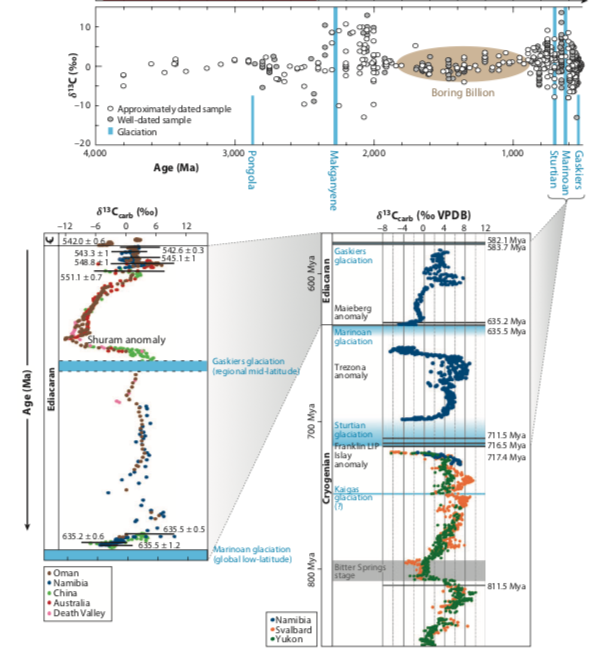
\includegraphics[width=.9\textwidth,height=.9\textheight,keepaspectratio]{img/pierrehumbert.png}
\end{frame}

\end{document}
